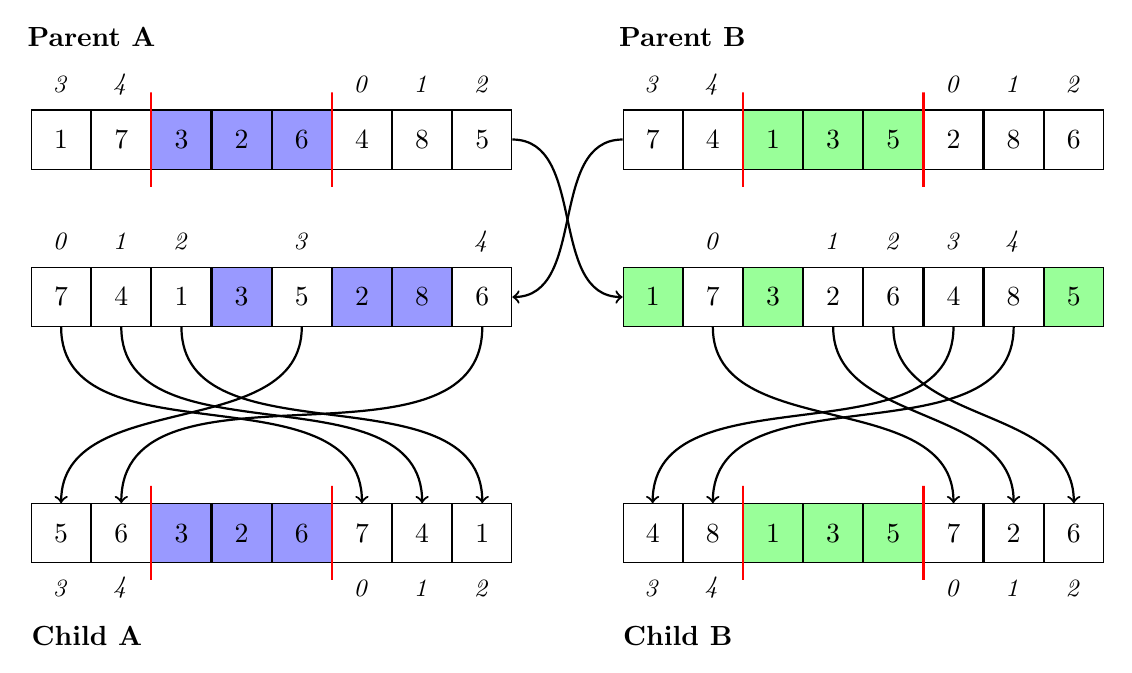
\begin{tikzpicture}
    % Define styles for the nodes
    \tikzstyle{cell} = [
        rectangle, text centered, draw,
        minimum width=0.75cm, minimum height=0.75cm
    ];

    \tikzstyle{index} = [
        text centered, font=\small, yshift=-0.3cm
    ];

    \tikzstyle{index_below} = [
        text centered, font=\small, yshift=0.3cm
    ];

    \tikzstyle{arrow} = [thick];

    % Parent A
    \node[cell]                             (a0)                {1};
    \node[cell, anchor=west]                (a1) at (a0.east)   {7};
    \node[cell, anchor=west, fill=blue!40]  (a2) at (a1.east)   {3};
    \node[cell, anchor=west, fill=blue!40]  (a3) at (a2.east)   {2};
    \node[cell, anchor=west, fill=blue!40]  (a4) at (a3.east)   {6};
    \node[cell, anchor=west]                (a5) at (a4.east)   {4};
    \node[cell, anchor=west]                (a6) at (a5.east)   {8};
    \node[cell, anchor=west]                (a7) at (a6.east)   {5};

    \node[
        anchor=west, xshift=-0.05cm, yshift=1.3cm, inner sep=0
    ] (parent_a) at (a0.west) {\textbf{Parent A}};

    \node[index, above of=a5] {\textit{0}};
    \node[index, above of=a6] {\textit{1}};
    \node[index, above of=a7] {\textit{2}};
    \node[index, above of=a0] {\textit{3}};
    \node[index, above of=a1] {\textit{4}};

    % Parent B
    \node[cell, anchor=west, xshift=1.4cm]  (b0) at (a7.east)   {7};
    \node[cell, anchor=west]                (b1) at (b0.east)   {4};
    \node[cell, anchor=west, fill=green!40] (b2) at (b1.east)   {1};
    \node[cell, anchor=west, fill=green!40] (b3) at (b2.east)   {3};
    \node[cell, anchor=west, fill=green!40] (b4) at (b3.east)   {5};
    \node[cell, anchor=west]                (b5) at (b4.east)   {2};
    \node[cell, anchor=west]                (b6) at (b5.east)   {8};
    \node[cell, anchor=west]                (b7) at (b6.east)   {6};

    \node[
        anchor=west, xshift=-0.05cm, yshift=1.3cm, inner sep=0
    ] (parent_b) at (b0.west) {\textbf{Parent B}};

    \node[index, above of=b5] {\textit{0}};
    \node[index, above of=b6] {\textit{1}};
    \node[index, above of=b7] {\textit{2}};
    \node[index, above of=b0] {\textit{3}};
    \node[index, above of=b1] {\textit{4}};


    % Cut Lines for A
    \draw[thick, red] (a1.east) -- ++(0cm,0.6cm) -- ++(0cm,-1.2cm);
    \draw[thick, red] (a4.east) -- ++(0cm,0.6cm) -- ++(0cm,-1.2cm);

    % Cut Lines for B
    \draw[thick, red] (b1.east) -- ++(0cm,0.6cm) -- ++(0cm,-1.2cm);
    \draw[thick, red] (b4.east) -- ++(0cm,0.6cm) -- ++(0cm,-1.2cm);

    % Parent B'
    \node[cell, anchor=west, yshift=-2cm]   (b'0) at (a0.west)    {7};
    \node[cell, anchor=west]                (b'1) at (b'0.east)   {4};
    \node[cell, anchor=west]                (b'2) at (b'1.east)   {1};
    \node[cell, anchor=west, fill=blue!40]  (b'3) at (b'2.east)   {3};
    \node[cell, anchor=west]                (b'4) at (b'3.east)   {5};
    \node[cell, anchor=west, fill=blue!40]  (b'5) at (b'4.east)   {2};
    \node[cell, anchor=west, fill=blue!40]  (b'6) at (b'5.east)   {8};
    \node[cell, anchor=west]                (b'7) at (b'6.east)   {6};

    \node[index, above of=b'0] {\textit{0}};
    \node[index, above of=b'1] {\textit{1}};
    \node[index, above of=b'2] {\textit{2}};
    \node[index, above of=b'4] {\textit{3}};
    \node[index, above of=b'7] {\textit{4}};

    % Parent A'
    \node[cell, anchor=west, xshift=1.4cm, fill=green!40]  (a'0) at (b'7.east)   {1};
    \node[cell, anchor=west]                (a'1) at (a'0.east)   {7};
    \node[cell, anchor=west, fill=green!40] (a'2) at (a'1.east)   {3};
    \node[cell, anchor=west]                (a'3) at (a'2.east)   {2};
    \node[cell, anchor=west]                (a'4) at (a'3.east)   {6};
    \node[cell, anchor=west]                (a'5) at (a'4.east)   {4};
    \node[cell, anchor=west]                (a'6) at (a'5.east)   {8};
    \node[cell, anchor=west, fill=green!40] (a'7) at (a'6.east)   {5};

    \node[index, above of=a'1] {\textit{0}};
    \node[index, above of=a'3] {\textit{1}};
    \node[index, above of=a'4] {\textit{2}};
    \node[index, above of=a'5] {\textit{3}};
    \node[index, above of=a'6] {\textit{4}};

    % Arrows
    \draw[->, thick, out=0, in=180] (a7.east) to (a'0.west);
    \draw[->, thick, out=180, in=0] (b0.west) to (b'7.east);

    % Child A
    \node[cell, anchor=west, yshift=-3.0cm] (ca0) at (b'0.west) {5};
    \node[cell, anchor=west]                (ca1) at (ca0.east) {6};
    \node[cell, anchor=west, fill=blue!40]  (ca2) at (ca1.east) {3};
    \node[cell, anchor=west, fill=blue!40]  (ca3) at (ca2.east) {2};
    \node[cell, anchor=west, fill=blue!40]  (ca4) at (ca3.east) {6};
    \node[cell, anchor=west]                (ca5) at (ca4.east) {7};
    \node[cell, anchor=west]                (ca6) at (ca5.east) {4};
    \node[cell, anchor=west]                (ca7) at (ca6.east) {1};

    \node[
        anchor=west, yshift=-1.3cm, inner sep=0
    ] (child_a) at (ca0.west) {\textbf{Child A}};

    \node[index_below, below of=ca5] {\textit{0}};
    \node[index_below, below of=ca6] {\textit{1}};
    \node[index_below, below of=ca7] {\textit{2}};
    \node[index_below, below of=ca0] {\textit{3}};
    \node[index_below, below of=ca1] {\textit{4}};

    % Child B
    \node[cell, anchor=west, xshift=1.4cm]  (cb0) at (ca7.east) {4};
    \node[cell, anchor=west]                (cb1) at (cb0.east) {8};
    \node[cell, anchor=west, fill=green!40] (cb2) at (cb1.east) {1};
    \node[cell, anchor=west, fill=green!40] (cb3) at (cb2.east) {3};
    \node[cell, anchor=west, fill=green!40] (cb4) at (cb3.east) {5};
    \node[cell, anchor=west]                (cb5) at (cb4.east) {7};
    \node[cell, anchor=west]                (cb6) at (cb5.east) {2};
    \node[cell, anchor=west]                (cb7) at (cb6.east) {6};

    \node[
        anchor=west, yshift=-1.3cm, inner sep=0
    ] (child_b) at (cb0.west) {\textbf{Child B}};

    \node[index_below, below of=cb5] {\textit{0}};
    \node[index_below, below of=cb6] {\textit{1}};
    \node[index_below, below of=cb7] {\textit{2}};
    \node[index_below, below of=cb0] {\textit{3}};
    \node[index_below, below of=cb1] {\textit{4}};

    % Cut Lines for Child A
    \draw[thick, red] (ca1.east) -- ++(0cm,0.6cm) -- ++(0cm,-1.2cm);
    \draw[thick, red] (ca4.east) -- ++(0cm,0.6cm) -- ++(0cm,-1.2cm);

    % Cut Lines for Child B
    \draw[thick, red] (cb1.east) -- ++(0cm,0.6cm) -- ++(0cm,-1.2cm);
    \draw[thick, red] (cb4.east) -- ++(0cm,0.6cm) -- ++(0cm,-1.2cm);


    % Children A - Arrows
    \draw[->, thick, out=270, in=90] (b'0.south) to (ca5.north);
    \draw[->, thick, out=270, in=90] (b'1.south) to (ca6.north);
    \draw[->, thick, out=270, in=90] (b'2.south) to (ca7.north);
    \draw[->, thick, out=270, in=90] (b'4.south) to (ca0.north);
    \draw[->, thick, out=270, in=90] (b'7.south) to (ca1.north);

    % Children B - Arrows
    \draw[->, thick, out=270, in=90] (a'1.south) to (cb5.north);
    \draw[->, thick, out=270, in=90] (a'3.south) to (cb6.north);
    \draw[->, thick, out=270, in=90] (a'4.south) to (cb7.north);
    \draw[->, thick, out=270, in=90] (a'5.south) to (cb0.north);
    \draw[->, thick, out=270, in=90] (a'6.south) to (cb1.north);

\end{tikzpicture}
